\documentclass[12pt]{article}
\usepackage{geometry}
\geometry{letterpaper, left=22.5mm, right=22.5mm, top=30mm, bottom=30mm}
\geometry{letterpaper}
\usepackage{amsmath}
\usepackage{amssymb}
\usepackage{enumitem}
\usepackage{fancyhdr}
\usepackage{framed}
\usepackage{tikz}
\usepackage{mathpazo}
%\usepackage{charter}
%\usepackage{newcent}
\usepackage{indentfirst}
\usepackage{booktabs}
\usepackage{graphicx}
\usepackage{float}
\usepackage{makecell}
\usepackage{xcolor}
\usepackage{mdframed}
\usetikzlibrary{trees}
\pagestyle{fancy}
\usepackage{amsthm}
\theoremstyle{definition}
\newtheorem{definition}{Definition}[section]
\theoremstyle{property}
\newtheorem{property}{Property}[section]
\theoremstyle{assumption}
\newtheorem{assumption}{Assumption}[section]
\theoremstyle{example}
\newtheorem{example}{Example}[section]
\theoremstyle{comment}
\newtheorem{comment}{Comment}[section]
\newtheorem{theorem}{Theorem}[section]
\newtheorem{corollary}{Corollary}[theorem]
\newtheorem{lemma}[theorem]{Lemma}
\usepackage{lastpage}
\usepackage{wrapfig}
\usepackage{hyperref}
\usepackage{subcaption}
\usepackage{setspace}
\hypersetup{
colorlinks=true,
linkcolor=black,
filecolor=green, 
urlcolor=blue,
}
% Additional decision tree setup %%
\usetikzlibrary{positioning}
\newdimen\nodeDist
\nodeDist=35mm

%%%
\newcommand{\ROM}[1]
    {\MakeUppercase{\romannumeral #1}}
    
    \DeclareMathOperator*{\plim}{plim}
\fancyhead[L]{Econometrics \ROM{2}: Recitation 13}%change each reci
\fancyhead[R]{Spring 2022}
\fancyfoot[C]{\thepage \hspace{1pt} / \pageref{LastPage}}

\fancypagestyle{firstpage}{%
\fancyhf{}%
\renewcommand{\headrulewidth}{0mm}%
  \fancyfoot[C]{\thepage \hspace{1pt} / \pageref{LastPage}}
}
%change title each rec
\title{Introduction to Econometrics \ROM{2}: Recitation 13}

\begin{document}
\linespread{1.25}
\onehalfspacing

\author{Seung-hun Lee\footnote{Contact me at \href{mailto:sl4436@columbia.edu}{sl4436@columbia.edu} if you spot any errors or have suggestions on improving this note.}}
\date{May 2nd, 2022}
\maketitle
\thispagestyle{firstpage}

%%%%%%%%%%%%%%%%%%

\section{Machine Learning}
\subsection{Decision trees}
We have an IID data $(y_i,x_i)$ for $i\in\{1,...,n\}$. Decision trees are used to represent decision making and algorithms behind classification problem (discrete $y_i$) or regression problems (continuous $y_i$). The basis function used here are represented in terms of splits and have nonlinear functions - indicators based on categorization of cutoff. Decision trees give us an intuitive interpretation behind decision-making procedures and invariant to monotonic transformations (based on features of the indicator function). 
\subsubsection{Classical decision trees: Classification and regression trees}
Classification and regression treeds (CART) describes a discrete variable regression or classification in the form of trees, with the goal of finding the algorithm that best predicts out-sample. The form of these trees are similar to game trees we observe in Game Theory. Key difference is that we populate each nodes with the decision criteria, rather than a player. and the path taken is determined by the results of a classification, usually a cutoff or categorization. 
\par
Before going forward, we need to clear some basic terminologies used in decision trees
\begin{itemize}
\item Branch: Path from one node to other
\item Split: Process of dividing a sample based on a criterion specified at a node; creates two branches per non-terminal nodes
\item Depth: Number of stages with splits
\item Leaves: Output; or nodes on the last stage
\item Pruning: Reducing the size of the tree (steps or fewer splits)
\end{itemize} \par
When the decision tree is first trained, it follows a recursive greedy algorithm. It is recursive in the sense that there are repeated nodes where there is a partitioning of two-way splits. Each time, we select a variable $x_k$ and threshold/class that allows each split outcome to be as different as possible. Formally speaking, we seek to maximize the between variance of outcome $y$ or increase the information gain. This process stops when the decision tree reaches certain depth, each leaf is desirably small, and additional information gain is small. The algorithm is greedy in that at each given non-terminal node, the best test selected is only locally optimal - so there is no forward looking aspect here. This is usually computationally cheaper because finding the optimal tree that maximizes predictive ability is $NP$-hard; It cannot be solved in a determined polynomial time and this leads to additional costs. \par
In determining the split, we try to find a split that gives us large between variance and information gain. Between variance measures the total variation between each group mean to the overall mean and is characterized as the $R^2$ of
\[
y=\beta\mathbb{1}(x_k>t)+u
\]
and is usually used in regression problem. This should be distinguished from within-group variation, which checks for the total variation in the individual values in each group and their respective group mean. High between variance indicates that the regression performs well in distinguishing factors that explain $y$. \par 
Information gain can be defined as follows for a potential split $S=S_1\cup S_2$ \par
\[
IG = L(S)-\left[\frac{|S_1|}{|S|}L(S_1)+\frac{|S_2|}{|S|}L(S_2)\right]
\]
where $L(C)=-\sum_{j=1}^J f_j \log{f_j}$ is the entropy and $f_j$ is the proportion of class $j$ in $C$. Depending on how we set up $S_1$ and $S_2$, we may have a classification that gives us more certainty (lower entropy at $S_1$ and $S_2$) or higher uncertainty (high entropy at $S_1$ and $S_2$). When we set the splits appropriately, we can find subsequent classifications where uncertainty is low at $S_1$ and $S_2$, which gives us a tree with better prediction. Information gain can be thought of as a metric that assess the informative properties of each split in a tree. \par
\begin{mdframed}[backgroundcolor=blue!5] 
\begin{definition}[Entropy in information theory] The entropy of a random variable $X$ is the average level of uncertainty inherent to the varianble's possible outcomes. Suppose $X$ has possible outcomes $x_1,...,x_n$, occurring at probabilities $p_1,...,p_n$. We write
\[
L(X)=-\sum_{i=1}^n p_i\log{p_i}
\]
This is high when events in the random variable are closer to equiprobable case. On the other hand, if there is only one possible event such that $p_1=1$ and $p_j=0\ \forall j\neq1$, the resulting entropy is 0. 
\end{definition}
\end{mdframed}\par
While decision trees may be informative, it is definitely not perfect. One problem comes from the selection of hyperparameters (or parameters whose value is used to control the learning process such as split criterion, stopping criteria). Improper selection of such hyperparameters are likely to lead to overfitting and bad out-sample predictions. One way to address this is to prune the tree - making the trees more compact by eliminating some splits - through cross-validation. Moreover, the greedy algorithm is not forward-looking. So the decision tree may not be stable and the most optimal possible, especially when the top node is incorrectly selected. 
\subsubsection{Bagging}
Bagging stands for `Boostrap AGGregatING'. It takes an idea from the ensemble method in that it averages from multiple decision trees to enhance stability and accuracy of prediction, classification, and regression. By averaging, bagging protects from overfitting the data and prevents instability. 
\par
The procedure is very similar to that of bootstrapping. They are as follows
\begin{enumerate}
\item Bootstrap: Let's have a sufficiently large $B$ resamples with replacement. In each resampling step, we fit a tree.
\item Aggregation: We average the predictions of the $B$ trees to predict $y$ given $x$. 
\end{enumerate}
So how do we assess the predictive capability of the model? That depends on the dispersion of the $B$ predictions from each resampling. Smaller dispersions imply that the prediction is likely to be more accurate than those with larger dispersion. 
\subsubsection{Random forests}
Random forests is a way of averaging multiple deep decision trees, trained on different parts of the same training data set. The goal here is to reduce the variance of the prediction. It uses ensemble method in that it averages multiple algorithms and at the surface, uses similar methods to bagging. Unlike bagging, random forests choose splits from a smaller number of randomly selected covariates at each step of the tree construction (this is sometimes called `feature bagging'). Typically, for the learning process with $k$ total features available, $\sqrt{k}$ is used in classification problems and $\max\{k/3,5\}$ is used in regression.
\par
 In doing this, each trees are less likely to be correlated than each other compared to earlier methods. In earlier methods, a feature with a strong explanatory power may be used in multiple trees, leading to high correlation between different trees. Also as a result, it is very likely that in random forests, the top splits are usually in different variables. 
 \par
Random forest does better than earlier methods in regards to preventing overfitting and stability. Moreover, random forests can be used to rank the importance of the variables by averaging the decline in the split-criterion (or the out-of-bag error before and after permutation over all $B$ tres). When this value is large (due to huge decline in the out-of-bag error), this variable can be considered important and can be used as a basis for variable selection. One key problem is that we lose interpretability. This is due to a black-box like procedure in the selection of the random subsample of covariates (and this is where variable importance analysis becomes essential here).  \par
An extension of the random forest is a causal forest (Wagner, Athey 2018), which uses random forests to estimate the treatment effect under the assumption of conditional independence (or unconfoundedness). We first estimate the propensity score $\hat{p}_i$ and transform $y_i$ into
\[
\hat{y}_i = \frac{D_i-\hat{p}_i}{\hat{p}_i(1-\hat{p}_i)}y_i
\]
This gives us the inverse probability weight formula. If $D_i=1$, we have $\hat{y}_i=\frac{1}{\hat{p}_i}y_i$. If $D_i=0$, we get $\hat{y}_i=\frac{1}{1-\hat{p}_i}y_i$. By taking the expected value of $\hat{y}_i$ we get
\[
\widehat{TE}(x)=E[\hat{y}_i|x]
\]
Once this is done, we can do an honest inference by estimating on a subsample that is different from the training and test subsamples. We can then do normal inference on $\widehat{TE}(x)$. Random forests are used in estimating for the propensity score and honest inference. $\hat{p}_i$ is obtained by the proportion of treated observations in the leaf of $x_i$ that comes from some random forest. Honest estimation is done by several types of random forest estimation - Double-sample trees (split sample to two - one is used to estimate $\mu(x,d)$ and the other is used to determine splits) is one of them. For further details, refer to Wagner, and Athey (2018).    \par
Another extension of the random forest is a local linear forest (Friedberg, Tibshirani, Athey, Wagner 2020). The idea behind local linear forests is to use a random forest to generate weights that can serve as a kernel for a local linear regression. Suppose that $y_i=m(X_i)+e_i$. Local linear forest method uses random forest to estimate the conditional mean function $m(x_0)$ at fixed test point $x_0$. Here, random forests are used as adaptive weight generators (not necessarily an ensemble method). Specifically,
\[
\hat{m}(x_0)=\frac{1}{B}\sum_{i=1}^n \sum_{b=1}^By_i \frac{\mathbb{1}[X_i\in L_b(x_0)]}{|L_b(x_0)|}=\sum_{i=1}^n y_i \underbrace{\frac{1}{B}\sum_{b=1}^B\frac{\mathbb{1}[X_i\in L_b(x_0)]}{|L_b(x_0)|}}_{\alpha_i(x_0)}
\]
Here, $L_b(x_0)$ represents the leaf at $b$'th tree, $|\cdot|$ indicates the size of the leaves (number of leaves in that tree). $\alpha_i(x_0)$ is the fraction of trees in which an observation appears in the same leaf as the target value of the covariate vector. Local linear forests solve the weighted least problem below with penalty term using the weights defined above
\[
\begin{pmatrix} \hat{m}(x_0) \\ \hat{\theta}(x_0) \end{pmatrix} = \arg\min_{m,\theta}\left[ \sum_{i=1}^n \alpha_i(x_0) (y_i-m(x_0)-(x-x_0)\theta(x_0))^2 +\lambda ||\theta(x_0)||^2\right]
\]
The value of local linear forest is that it allows us to use local linear regressions in high-dimensions with a meaningful kernel and predict with random forests even in the presence of smooth, strong signals (Random forests are known to not perform well in the presence of strong and smooth effects). So it overcomes the weakness of the nonparametric estimation (curse of dimensionality) and random forests for better prediction and confidence intervals. 
\subsubsection{Gradient-boosted trees}
Like gradient boosting, we start with weak learners - trees with shallow depth, in our context. We seek to improve their performance on the observation they misclassify by boosting the weight of these observations. The performance will be measured by minimization of a loss function. So we write the objective function as
\[
\min \sum_{i=1}^n L(y_i,\hat{y}_i), \ \text{say, } (y_i-\hat{y}_i)^2
\] 
We do this as follows: Let $v(x,S)$ be the average value of $y$ in the leaf that contains $x$ in a shallow tree with splits $S$. Let $d$ be some small number to represent a shallow decision tree. Then we proceed in these steps
\begin{enumerate}
\item Begin with an initial prediction: $\hat{y}_i^{(0)}=E[y_i]$
\item For each iteration $b\in\{1,...,B\}$, we choose split $S_b$ in the tree of depth $d$ to minimize
\[
\sum_{i=1}^n L(y_i, \hat{y}_i^{(b-1)}+v(x_i,S) )
\]
and update our prediction $\hat{y}_i^{(b)}= \hat{y}_i^{(b-1)}+\epsilon v(x_i,S_b)$. Note that $\epsilon$ is the learning rate and is not $\epsilon=1$, which would mean updating the prediction by the exact value and risk overshooting
\end{enumerate}\par
We can also tune the model by including a complexity penalty in the loss function. So when we minimize, the objective function when choosing the split $S_b$ is (need to do this for many trees)
\[
\sum_{i=1}^n L(y_i, \hat{y}_i^{(b-1)}+v(x_i,S) ) + C(S)
\]\par
An even improved version of gradient boosted trees is called XGBoost algorithm (Extreme gradient boosting). It is extreme in the sense that it implements gradient boosting procedure at a highly efficient, flexible rate (computationally) compared to older gradient boosting methods. This is achieved by introducing a quadratic loss and complexity penalty functions, which are computationally easier to deal with. The new version of the objective function is
\[
\sum_{i=1}^n (G_iv(x_i, S)+\frac{1}{2} H_i v(x_i,S)^2)+ \gamma K + \frac{\lambda}{2}\sum_{k=1}^K v_k^2
\]
where $G_i$ and $H_i$ are each the first and second derivatives of the $L(y_i. \hat{y}_i)$ w.r.t $\hat{y}_i$ at $(y_i, \hat{y}_i^{(b-1)})$, $K$ is the number of leaves, and $v_k$ is the predictor on leaf $k$. \par
This process can help us characterize the closed-form formula for the optimal predictors $v_k$ at a much faster rate. There are still some heavy-lifting to do in that we still have to construct the tree using recursive partitioning. We also need to select the number of leaves $K$, so we still need tuning. 

\subsection{Artificial neural networks}
In general, artificial neural networks refer to a computational system that resembles biological neural networks - there is an input that transmits signals, output, and intermediary nodes which processes a signal received from earlier nodes and generates the signals to later nodes. A simple diagram of artificial neural network can be described as follows:

\begin{figure}[H]
\centering
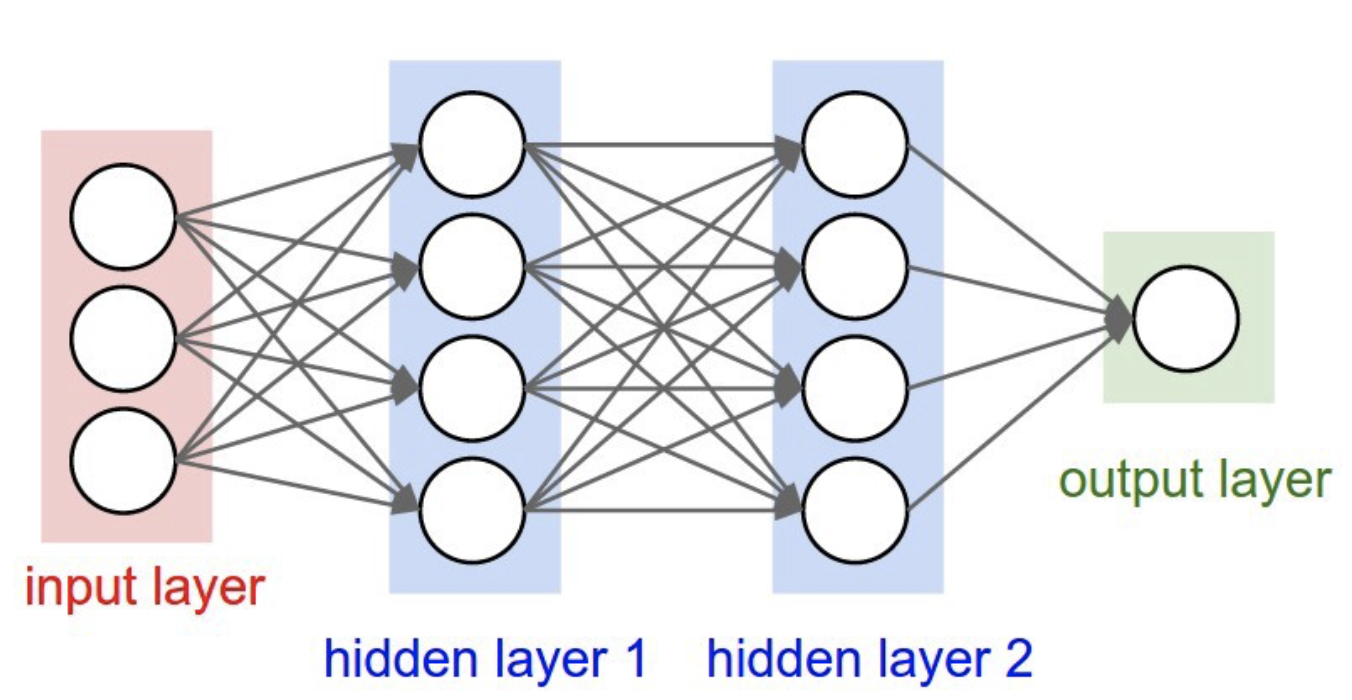
\includegraphics[width=0.8\textwidth, keepaspectratio]{neuralnetwork.png}
\end{figure}
\par
In our context, inputs can be thought of as covariates, the lines between layers being weighted by some $w$ coefficients, and lines to the output layer represents signal $\sigma(\cdot)$, which is called an activation function. These activation signals takes a specific form, such as a sigmoid function (logistic CDF), multinomial logit (or softmax), or a rectified linear unit function (ReLU, with $\sigma(t)=\max\{0,t\}$) \par
\subsubsection{Single hidden layer neurons (Single-layer perception)}
Suppose we limit ourselves to a single hidden layer. There are $M$ neurons in the input layer, and $L$ nodes in the hidden layer. Input neurons are denoted $x_1,...,x_M$ have weights $w_{1lm},\ m\in\{1,...,M\},\ l\in\{1,...,L\}$, and emit $\sigma(\sum_{m} w_{1lm}x_m)$ to a hidden layer $l$. The hidden layer has its own weight for each node, $w_{2l}$, which are used to combine inputs from previous nodes to generate a prediction for the output node $\hat{y} = g\left(\sum_l w_{2l}\sigma(\sum_{m} w_{1lm}x_m)\right)$, where $g(\cdot)$ is the activation function for the output layer. In case of regressions $g(t)=t$, where as a classification into $K$ categories uses a softmax function as an activation function. \par
In fitting a single-layer perception, we iterate forward starting from the input to the output node and than iterate backward per run, or epoch. We start from the forward pass. Given a loss function $L(y,\hat{y}(\theta))$ and an initial value of $\theta=(w_1, w_2)$, we compute
\[
z_{il}=\sigma(w_{1l}'x_i)
\]
and then the output can be produed as
\[
\hat{y}_i(\theta) = w_2'z_i = \sum_l w_{2l}\sigma\left(\sum_{m} w_{1lm}x_{im}\right)
\] \par
In the backward pass, we compute the components of the loss functions, then take gradients with respect to elements in $\theta$, and do approximate Newton iteration:
\[
\theta^{(s+1)}=\theta^{(s)}-\epsilon_s\frac{\partial L}{\partial \theta}(\theta^{(s)})
\]
which can be conducted similar to gradient descent methods such as minibatch descent. $\epsilon_s$ is the learning rate which ideally should goes to 0. The problem here is that there may be so many elements in $\theta$, leading to challenges in terms of efficiently updating these values correctly.  This is where backpropagation come in. This is, to put it very simply, an automated differentiation and application of chain rule to identify gradients used to update the values of the weights. We start from the output and update the $w_2$ first using
\[
\frac{\partial L}{\partial w_{2l}}(\theta^{(s)}) = -2 \sum_{i=1}^n (y_i-\hat{y}_i^{(s)}(\theta))z_{il}
\]
and Newton iteration method. We then move further back to update $w_1$ using
\[
\frac{\partial L}{\partial w_{1lm}}(\theta^{(s)}) = -2 \sum_{i=1}^n (y_i-\hat{y}_i^{(s)}(\theta))x_{im}\sum_{l}\mathbb{1}((w_l^{(s)})'x_i>0 ))
\]
where we have assume $\sigma(t)=\max\{0,t\}$ for this exercise. 
\subsubsection{Deep learning}
This is a case where we have two or more hidden layers, and each nodes are fully connected. This means that there are so much more parameters, activation functions, and hyperparameters (learning rate and epoch) to choose. Suppose that we have $p$ covariates, $K$ outputs, $D$ hidden layers, and $M$ nodes per layer. We are given $p$ and $K$, so we need to make a decision on how many neurons to have per layer and the depth of our artificial neural network. In total, we have $pM + (D-1)M^2 + kM$ parameters (or weights) to work with. \par
In general, what is known is that it is better to have a deep artificial neural networks than wider ones. Small $D$ has trouble fitting well, but too large $D$ is better if many weights are small, despite rising chances of overfitting. To avoid overfitting, we can minimize a loss function $L(\theta)$ which also includes a penalty term $\lambda ||\theta||_q^q$.

\par
 One drawback is that cross-validation will be too costly with deep learning due to the bulk of the load it has to work on with so many parameters and hyperparameters. As an alternative, we can do a dropout method. This method randomly eliminates some links and thins the neural networks, which is then retrained and tested/compared with all the eliminated units brought back in. 
\par
So what other reasons do we have in preferring a deeper tree? If not, we would need to resort to a shallower tree with many number of units, which does poorly compared to deeper ones. Also, deeper trees do better in terms of expressiveness - much more various and complex functions can be expressed with deeper networks than in shallower ones. 

\subsubsection{Application to treatment effects: Double machine learning debiasing techniques}
One use of deep learning methods is in finding the ATE under the assumption of conditional independence. Write our setup as
\[
y_ i = \mu(X_i, D_i)+\epsilon_i(D_i), \ D_i=\mathbb{1}(u_i<p(X_i))
\]
and $(\epsilon(0), \epsilon(1))\perp\!\!\perp u|X$. In principle, we can use machine learning techniques to estimate the propensity score $p(X_i)$ and $\mu(X_i, D_i)=E[y_i|D_i, X_i]$ and use this to calculate an inverse-probability weighted ATE.
\par
One technique used in this aspect is the double machine learning debiasing technique by Chernozhukov et al (2018). The reason why debiasing is involved here is because of the $p(X_i)$ and $\mu$. These are nuisance parameters whose errors can affect our estimate of the treatment effect. So we need to debias the TE by decoupling the TE from the $p(X_i)$ and $\mu$ using Neyman orthogonalization that block-diagonalizes the (Fisher) information matrix. A nonzero nondiagonal element implies that determining TE also depends on nuisance parameters. Chernozhukov et al (2018) shows how this decoupling methods can be carried out using machine learning methods. 
\par
Briefly speaking, we split the sample data into $K$ folds, then we leave one of the folds out and use LASSO (or other methods) to estimate the propensity score $\hat{p}_k=\Pr(D=1|X)$. Next, we take the Neyman-orthogonalized combination of the estimates of $p(X_i)$ and $\mu$. The estimator that comes out from here has standard asymptotics assuming that the functions are smooth enough (converge quicker than $n^{-1/4}$). This allows us to do standard tests on our estimates. 
%%%%%%%%%%%%%%%
\end{document}

